\documentclass[a4paper,11pt,usenames,dvipsnames]{article}
\usepackage{times}

\usepackage{fullpage} 

\usepackage{ifpdf} 

\ifpdf
\usepackage[pdftex]{graphicx}
\usepackage[pdftex,pdftitle={Kinematic Particle Code User Guide},
               pdfauthor={J.~Threlfall},
               pdfsubject={User Guide},
               pdfkeywords={},linktocpage=true,citecolor=red,linkcolor=blue,
                pdfpagemode={Fullscreen},bookmarks=false,bookmarksopen=false,
                colorlinks=true]{hyperref}
\else
\usepackage{graphicx}
\fi 

\ifpdf
\DeclareGraphicsExtensions{.pdf,.jpg,.tif}
\else
\DeclareGraphicsExtensions{.eps,.jpg}
\fi

\usepackage{natbib}
\bibpunct{(}{)}{;}{a}{}{,} % to follow the A&A style
\usepackage{color}
\usepackage{enumitem}
\usepackage{amssymb}	% extra maths symbols
\usepackage{amsmath}
\usepackage{courier}
\usepackage{aas_macros}	% macros for bibliography
\usepackage{subfig}  	% subfigure support
\usepackage{epsfig}	% epsfigs
\usepackage{cancel}

\graphicspath{{figs/}}
% This is my horrible mutated version of Claire Parnell's original math_def.tex file
% It hopefully contains lots of useful shortcuts, defined to make life easier..
% Oh and I stuck in some stuff from Bernie's analytical project too...


\newcommand{\diff}[2]{\frac{{\rm d}#1}{{\rm d}#2}}
\newcommand{\ndiff}[3]{\frac{{\rm d}^{#3}#1}{{\rm d}#2^{#3}}}
\newcommand{\pdiff}[2]{\frac{\partial #1}{\partial #2}}
\newcommand{\npdiff}[3]{\frac{\partial^{#3} #1}{\partial #2^{#3}}}
\newcommand{\e}[1]{\ensuremath{{\rm e}^{#1}}}
\newcommand{\ldiff}[2]{\ensuremath{{\rm d}#1/{\rm d}#2}}
\newcommand{\lpdiff}[2]{\ensuremath{\partial#1/\partial#2}}
\newcommand{\lnpdiff}[3]{\ensuremath{\partial^{#3}#1/\partial#2^{#3}}}

\newcommand{\vel}{ {\bf v} }
\newcommand{\Efi}{ {\bf E} }
\newcommand{\Bfi}{ {\bf B} }
\newcommand{\Afi}{ {\bf A} }
\newcommand{\rfi}{ {\bf r} }
\newcommand{\dipm}{ {\bf m} }
\newcommand{\Mag}{ {\bf M} }
\newcommand{\Hfi}{ {\bf H} }
\newcommand{\Dfi}{ {\bf D} }
\newcommand{\rvec}{ {\bf r} }
\newcommand{\Icur}{ {\bf I} }
\newcommand{\Kcur}{ {\bf K} }
\newcommand{\Jcur}{ {\bf J} }
\newcommand{\rvechat}{ {\bf{\hat r}} }
\newcommand{\ulin}{ \underline }
\newcommand{\beq}{ \begin{eqnarray} }
\newcommand{\eeq}{ \end{eqnarray} }
\newcommand{\dl}{ {\rm d}l }
\newcommand{\da}{ {\rm d}a }
\newcommand{\dt}{ {\rm d}\tau }
\newcommand{\bdl}{ {\bf{\rm d}l} }
\newcommand{\bda}{ {\bf{\rm d}a} }
\newcommand{\bdt}{ {\bf{\rm d}\tau} }
\newcommand{\nor}{ {\bf n} }
\newcommand{\rmd}{ {\rm d} }
\newcommand{\dR}{ {\rm d}R }
\newcommand{\dth}{ {\rm d}\theta }
\newcommand{\dphi}{ {\rm d}\phi }
\newcommand{\lra}{ \longrightarrow }
\newcommand{\Lra}{ \Longrightarrow }

\newcommand{\xhat}{ {{\bf{\hat x}}} }
\newcommand{\yhat}{ {{\bf{\hat y}}} }
\newcommand{\zhat}{ {{\bf{\hat z}}} }
\newcommand{\rhat}{ {\bf{\hat r}} }
\newcommand{\Rhat}{ {\bf{\hat R}} }
\newcommand{\that}{ {\boldsymbol{\hat \theta}} }
\newcommand{\phat}{ {\boldsymbol{\hat \phi}} }
\newcommand{\dive }{ {\bf {\nabla}} \cdot }
\newcommand{\curl }{ {\bf {\nabla}} \times }
\newcommand{\lap }{ {\bf\nabla}^2 }
\newcommand{\parx}{ {\partial x} }
\newcommand{\pary}{ {\partial y} }
\newcommand{\parz}{ {\parital z} }
\newcommand{\parR}{ {\partial R} }
\newcommand{\parp}{ {\partial \phi} }
\newcommand{\parr}{ {\partial r} }
\newcommand{\pt}{ {\partial \theta} }
\newcommand{\dxdt}{ \frac{dx}{dt} }
\newcommand{\dydt}{ \frac{dy}{dt} }
\newcommand{\dzdt}{ \frac{dz}{dt} }
\newcommand{\ddxdt}{ \frac{d^2x}{dt^2} }
\newcommand{\ddydt}{ \frac{d^2y}{dt^2} }
\newcommand{\ddzdt}{ \frac{d^2z}{dt^2} }
\newcommand{\dddxdt}{ \frac{d^3x}{dt^3} }
\newcommand{\dddydt}{ \frac{d^3y}{dt^3} }
\newcommand{\dddzdt}{ \frac{d^3z}{dt^3} }
\newcommand{\drdtl}{ {d\bf{r}}/{dt}  }
\newcommand{\drdt}{ \frac{d \bf{r}}{dt}  }
\newcommand{\ddrdt}{ \frac{d^2 \bf{r}}{dt^2}  }
\newcommand{\dddrdt}{ \frac{d^3 \bf{r}}{dt^3}  }
\newcommand{\vpar}{ v_{\parallel} }
\newcommand{\vperp}{ v_{\perp} }
\newcommand{\Eperp}{ E_{\perp} }
\newcommand{\Wpar}{ W_{\parallel} }
\newcommand{\Wperp}{ W_{\perp} }
\newcommand{\dvdt}{ \frac{d \bf{v}}{dt}  }
\newcommand{\dvxdt}{ \frac{dv_x}{dt} }
\newcommand{\dvydt}{ \frac{dv_y}{dt} }
\newcommand{\dvzdt}{ \frac{dv_z}{dt} }
\newcommand{\ddvxdt}{ \frac{d^2v_x}{dt^2} }
\newcommand{\ddvydt}{ \frac{d^2v_y}{dt^2} }
\newcommand{\ddvzdt}{ \frac{d^2v_z}{dt^2} }
\newcommand{\dvx}{ \.v_x }
\newcommand{\dvy}{ \.v_y }
\newcommand{\dvz}{ \.v_z }
\newcommand{\ddvx}{ \"v_x }
\newcommand{\ddvy}{ \"v_y }
\newcommand{\ddvz}{ \"v_z }
\newcommand{\dOdy}{ \frac{ d \Omega}{dy}}
\newcommand{\dOp}{ \Omega_{o}^{'} }
\newcommand{\dOyp}{ \Omega_{y}^{'} }
\newcommand{\ddvxpdt}{ \frac{d^2}{dt^2} \left( v_{x0} + v_{x1} \right) }
\newcommand{\ddvypdt}{  \frac{d^2}{dt^2} \left( v_{y0} + v_{y1} \right) }
\newcommand{\ddvxldt}{ \frac{d^2v_{x0}}{dt^2} }
\newcommand{\ddvyldt}{ \frac{d^2v_{y0}}{dt^2} }
\newcommand{\ddvxsdt}{ \frac{d^2v_{x1}}{dt^2} }
\newcommand{\ddvysdt}{ \frac{d^2v_{y1}}{dt^2} }
\newcommand{\vxp}{\left( v_{x0} + v_{x1} \right) }
\newcommand{\vyp}{\left( v_{y0} + v_{y1} \right) }

\newcommand{\boldnabla}{\mbox{\boldmath$\nabla$}}

%Definitions used by Roberts

\def\A{{Alfv\'en}}
\def\Amp{Amp\`ere}
\def\Aic{Alfv\'enic}
\def\eq{equation}
\def\eqs{equations }
\def\mhd{magnetohydrodynamic }
\def\mhds{magnetohydrodynamics }
\def\ma{magnetoacoustic }
\def\azimorder{\rm n}
\def\w{\omega}
\def\ww{\omega^2}
\def\cs{c_s}
\def\css{c_s^2}
\def\cse{c_{se}}
\def\csse{c_{se}^2}
\def\cc{c^2}
\def\ca{{c_A}}
\def\caa{c_A^2}
\def\cao{c_{A}}
\def\caao{c_{A}^2}
\def\co{c_{s}}
\def\coo{c_{s}^2}
\def\cf{c_f}
\def\cff{c_f^2}
\def\ct{c_t}
\def\ctt{c_t^2}
\def\cto{c_{t}}
\def\ctto{c_{t}^2}
\def\ck{c_k}
\def\ckk{c_k^2}
\def\ce{c_{se}}
\def\cee{c_{se}^2}
\def\cae{c_{Ae}}
\def\caae{c_{Ae}^2}
\def\cte{c_{te}}
\def\ctte{c_{te}^2}
\def\rhoo{{\rho}_{0}}
\def\rhoe{{\rho}_{e}}
\def\Bo{B_{0}}
\def\Boo{B_{0}^{2}}
\def\Be{B_{e}}
\def\kz{k_z}
\def\kzz{k_z^2}
\def\kk{k^2}
\def\kms{km s$^{-1}$}
\def\Ws{\Omega_{saus}}
\def\Wss{\Omega_{saus}^{2}}
\def\nus{\nu_{saus}}
\def\Ps{P_{saus}}
\def\Wk{\Omega_{k}}
\def\Wkk{\Omega_{k}^{2}}
\def\nuk{\nu_{k}}
\def\Pk{P_{k}}
\def\Wac{\Omega_{ac}}
\def\Wacc{\Omega_{ac}^{2}}
\def\WA{\Omega_{A}}
\def\WAA{\Omega_{A}^{2}}
\def\nuA{\nu_{A}}
\def\PA{P_{A}}

\def\grad{\boldnabla}

% My Own Personal Additions:
\def\eo{\epsilon_{0}}
\def\muo{\mu_{0}}
\def\kpar{{k_{\parallel}}}
\def\kper{{k_{\perp}}}
\def\vxx{{\bf{v}_x}}
\def\vyy{{\bf{v}_y}}
\def\vzz{{\bf{v}_z}}
\def\vx{v_x}
\def\vy{v_y}
\def\vz{v_z}
\def\xhat{\bf{\hat{x}}}
\def\yhat{\bf{\hat{y}}}
\def\zhat{\bf{\hat{z}}}
\def\vhat{\hat{v}}
\def\di{\delta_i}

\def\vscl{{\color{OliveGreen}{v_{scl}}}}
\def\vsclsq{{\color{OliveGreen}{{v_{scl}}^2}}}
\def\lscl{{\color{OliveGreen}{l_{scl}}}}
\def\tscl{{\color{OliveGreen}{t_{scl}}}}
\def\bscl{{\color{OliveGreen}{b_{scl}}}}
\def\escl{{\color{OliveGreen}{e_{scl}}}}
\def\enscl{{\color{OliveGreen}{en_{scl}}}}
\def\omscl{{\color{OliveGreen}{\Omega_{e}^{scl}}}}
\def\muscl{{\color{OliveGreen}{\mu_{scl}}}}

\newcommand{\angstrom}{\mbox{\normalfont\AA}}
\newcommand{\Epar}{E_{\parallel}}
\newcommand{\upar}{u_{\parallel}}
\newcommand{\ue}{{{\bf{u}}_E}}
\newcommand{\ugb}{{\bf{u}}_{\grad{B}}}
%\def\o{c_{A0}}
%\def\caao{c_{A0}^2}
%\def\co{c_{0}}
%\def\coo{c_{0}^2}
%\def\cto{c_{t0}}
%\def\ctto{c_{t0}^2}
%EndDefinitions
   


\begin{document}
\title{
\bfseries\scshape Kinematic particle code - User Guide}
\author{\bfseries\itshape James Threlfall\thanks{E-mail address: jamest@mcs.st-and.ac.uk}, Thomas Neukirch, Paolo Guiliani \\
School of Mathematics and Statistics, University of St Andrews,\\
St Andrews, Fife, KY16 9SS, U.K.}
\date{November 2013}
\maketitle

\thispagestyle{empty}

 \section*{Abstract}
 We describe a numerical model designed to study the kinematic behaviour of individual particles in a magnetic field which obeys Ohm's law, using both relativistic and non-relativistic forms of the guiding centre approximation. This document describes how to obtain and run the code, the structure of the code itself, and various IDL scripts designed to aid data analysis. The contents of this document are aimed at code-users rather than developers. Lets do some science!

 \begin{center}
 \line(1,0){250}
 \end{center}

\section{Introduction}\label{sec:intro}
 The code is a modification of that used to study particle motion in collapsing magnetic trap (CMT) models of the solar atmosphere. Initial details (and scientific results from the initial CMT investigation) can be found in \citet{paper:Guilianietal2005}; the scheme has since been used in other investigations of CMT models \citep{paper:GradyNeukirch2009,paper:Gradyetal2012}. The code itself can be broadly split into two parts; a global (large/MHD-scale) field is required within which individual particle dynamics are calculated. While CMT models use a time-dependent transformation to a Lagrangian frame of reference to mimick post-flare loop "shrinkage", we have employed a large scale time-dependent model of magnetic reconnection in the presence of a separator, based on the work of \citet{paper:Wilmot-SmithHornig2011}. We have also included modules to allow the global field to be determined by the output of a {\tt{LareXd}} simulation \citep[see e.g.][]{paper:LareXd2001}. The latest version of our code can be downloaded from:

{\small \url{http://www-solar.mcs.st-andrews.ac.uk/~jamest/files/rnrcode_v2.tar.gz}}.

\section{Equations and normalisation}\label{sec:norm}
We will now describe the normalisation of both the global fields in our separator reconnection model and the equations which describe particle dynamics. By illustrating the normalisation of the separator reconnection field, we of course assume that if other global field configurations (e.g. CMT fields, test fields or fields determined through the {\tt{Lare}} plugin) are normalised in a similar way.

\subsection{Global field}
We base our global separator field model on the model of \citet{paper:Wilmot-SmithHornig2011}; the global separator field is formed by a potential magnetic field of the form 
 \begin{equation*}
  {\bf{B}}_0=\frac{b_0}{L^2}\left[x(z-3z_0){\xhat}+y(z+3z_0){\yhat}+\frac{1}{2}\left( z_0^2-z^2+x^2+y^2\right) {\zhat} \right], 
 \end{equation*}
 with magnetic null points at $\pm{z_0}$, while $b_0$ and $L$ determine the characteristic field strength and lengthscale of the model. For the original (essentially scale-free) model of \citet{paper:Wilmot-SmithHornig2011}, $z_0=5$, $b_0=1$ and $L=1$.
  \begin{figure*}[t]
   \centering
   \resizebox{0.4\textwidth}{!}{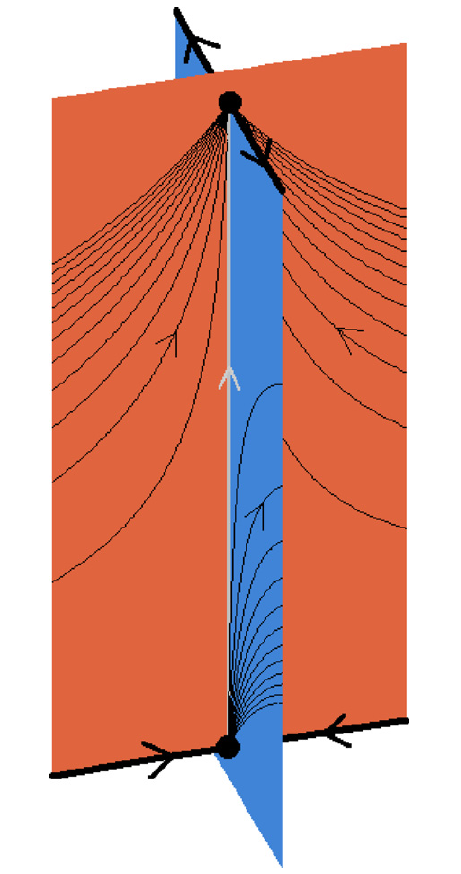
\includegraphics{Wilmot-SmithHornig_Fig1.png}} 
   \caption{Original magnetic configuration of the model of \citet{paper:Wilmot-SmithHornig2011}; the fan plane of the upper (lower) null is seen in orange (blue) and a separator (white) links both nulls at the intersection of the fan planes.} 
   \label{fig:WS}
  \end{figure*}
The null at $(0,0,-z_0)$ is classified as a \emph{positive null}, while that at $(0,0,+z_0)$ is a \emph{negative null} (due to the orientation of the magnetic field along the spine and fan of each null). The magnetic separator is formed by the intersection of the two fan planes associated with each null. The separator and general field configuration can be seen in Fig.~\ref{fig:WS}. 

With Faraday's Law coupling (time-varying) magnetic and electric fields, introducing a ring of magnetic flux of the form
\begin{align*}
 {\bf{B}}_{r}=\curl{\left[b_1 a \exp{\left(-\frac{\left( x-x_c\right)^2}{a^2}-\frac{\left( y-y_c\right)^2}{a^2}-\frac{\left( z-z_c\right)^2}{l^2} \right){\zhat} } \right] },
\end{align*}
(centred on $(x_c,y_c,z_c)$, with radius (in the $xy$ plane) controlled by the parameter $a$, the height (in $z$) by $l$ and the field strength by $b_1$) induces an electric field along the separator with the form
\begin{align*}
 {\bf{E}}=-\frac{b_1 a}{\tau}\exp{\left(-\frac{(x-x_c)^2}{a^2}-\frac{(y-y_c)^2}{a^2}-\frac{(z-z_c)^2}{l^2} \right) }{\zhat}.
\end{align*}
(provided that the time evolution satisfies Faraday's Law, i.e. that
\begin{align*}
 {\bf{B}}={\bf{B}}_0+\frac{t}{\tau}{\bf{B}}_{r}, \qquad 0\leq t\leq\tau,
\end{align*}
taking place over a timescale $\tau$).

We will input variables into the code in dimensional form, but the core equations use dimensionless variables. By choosing a normalising g magnetic field $\bscl$, lengthscale $\lscl$ and timescale $\tscl$, we may therefore relate dimensional and dimensionless quantities through
\begin{align*}
{\bf{B}}&=\bscl\,\bar{\bf{B}}, \qquad x=\lscl\,\bar{x}, \qquad t=\tscl\,\bar{t}.
\end{align*}
These three basic normalising quantities also determine how velocity, electric field and energy are scaled within the code:
\begin{align*}
 \vscl=\frac{\lscl}{\tscl}, \qquad \escl=\frac{\bscl\,\lscl}{\tscl}=\bscl\,\vscl, \qquad \enscl=\frac{1}{2}m{\vscl}^2,
\end{align*}
(where, for example, assessing the dimensions of Faraday's Law allows us to relate the electric field with our chosen quantities).

Therefore, the system of equations representing the behaviour of the global field structure is obtained as follows (where we have dropped the bar notation for system variables):
\begin{subequations}
\begin{align}
 {\bf{B}}_0&=\bar{b_0}\left[x\left( z-3\bar{z_0}\right){\xhat}+y\left( z+3\bar{z_0}\right) {\yhat}+\frac{1}{2}\left( \bar{z_0}^2-z^2+x^2+y^2\right) {\zhat} \right], \label{subeq:B0}  \\
{\bf{B}}_r&=\frac{2\bar{b_1}}{\bar{a}}\left[-y{\xhat}+x{\yhat}\right]\exp{\left(-\frac{(x-\bar{x_c})^2}{\bar{a}^2}-\frac{(y-\bar{y_c})^2}{\bar{a}^2}-\frac{(z-\bar{z_c})^2}{\bar{l}^2} \right)} , \label{subeq:Br}  \\
 {\bf{B}}&={\bf{B}}_0+\frac{{t}}{\bar{\tau}}{\bf{B}}_r, \qquad 0\leq t\leq\bar{\tau}, \label{subeq:B} \\
{\bf{E}}&=-\frac{\bar{b_1} \bar{a}}{\bar{\tau}}\exp{\left(-\frac{({x}-\bar{x_c})^2}{\bar{a}^2}-\frac{({y}-\bar{y_c})^2}{\bar{a}^2}-\frac{({z}-\bar{z_c})^2}{\bar{l}^2} \right) }{\zhat}, \label{subeq:E} 
\end{align}
\label{eq:fieldequations}
\end{subequations}
with $\bar{b_0}=\dfrac{b_0}{\bscl}$, $\bar{z_0}=\dfrac{z_0}{\lscl}$, $\bar{b_1}=\dfrac{b_1}{\bscl}$, $\bar{a}=\dfrac{a}{\lscl}$, $\bar{l}=\dfrac{l}{\lscl}$, $\bar{\tau}=\dfrac{\tau}{\tscl}\left( =\bar{t}_{\rm max}\right) $, $\dfrac{\bar{b_1}\bar{a}}{\bar{\tau}}=\dfrac{b_1a}{\tau\escl}$.

\subsection{Non-relativistic particle dynamics}\label{subsec:nonrel}
Having now established the global environment into which these particles will be inserted, we briefly turn our attention to the details of the particle motion itself. The drift equations solved by the code are based upon \cite{book:Northrop1963}:
\begin{subequations}
\begin{align}
 \frac{d\vpar}{dt}&=\frac{q\Epar}{m_0}-\frac{\mu_B}{m_0}\frac{\partial B}{\partial s}+
 \ue\cdot\left(\frac{\partial{\bf{b}}}{\partial t}+\vpar\frac{\partial{\bf{b}}}{\partial s}+\left( \ue\cdot\grad\right) {\bf{b}}\right), \label{eq:N1} \\
\dot{\bf{R}}_\perp&=\frac{\bf{b}}{B}\times\left[-{\bf{E}}+\frac{\mu_B}{q}\grad B+\frac{m_0}{q}\left(\vpar\frac{\partial{\bf{b}}}{\partial t}+\vpar^2\frac{\partial{\bf{b}}}{\partial s}\right.\right. \nonumber \\ 
&\qquad\qquad\qquad\left.\left.+\vpar\left( \ue\cdot\grad\right) {\bf{b}}+\frac{\partial\ue}{\partial t}+\vpar\frac{\partial \ue}{\partial s} +\left( \ue\cdot\grad\right) {\ue}\right)  \right], \label{eq:N2} \\
\frac{d}{dt}E_K&=q{\bf{\dot{R}}}\cdot{\bf{E}}+\mu_B\frac{\partial B}{\partial t}, \label{eq:N3} \\
E_K&=\frac{m_0{\vpar}^2}{2}+\mu_BB+\frac{m_0{u_E}^2}{2}, \label{eq:N4}
\end{align}
\label{eq:nrel}
\end{subequations}
where $\mu_B=1/2mv_g^2/B$ is the magnetic moment for a particle with gyro-velocity $v_g$, subject to ${E}\times{B}$ drift velocity $\ue(={\bf{E}}\times{\bf{b}}/B)$, ${\bf{b}}(={\bf{B}}/B)$ is the unit vector in the direction of the local magnetic field, ${\bf{R}}$ is the vector location of the guiding centre, $\vpar(={\bf{b}}\cdot{\dot{\bf{R}}})$ and $\Epar(={\bf{b}}\cdot{\bf{E}})$ are the magnitudes of the velocity and electric field parallel to the local magnetic field, $\dot{\bf{R}}_\perp(=\dot{\bf{R}}-\vpar{\bf{b}})$ is the component of velocity perpendicular to ${\bf{b}}$, and $s$ is a line element parallel to ${\bf{b}}$. We will only consider electrons in our model, thereby fixing mass $m=1.9\times10^{-31}\rm{kg}$ and charge $q=|e|=1.6022\times10^{-19}\rm{C}$.

Non-dimensionalising the first of these equations (and remembering that $\bf{b}$ is a unit vector, and as such has no units, i.e. ${\bf{b}}\equiv\bar{\bf{b}}$) proceeds as follows
\begin{align*}
 \frac{\vscl}{\tscl}\frac{d\bar{\vpar}}{d\bar{t}}&=\frac{q}{m}\escl\bar{\Epar}-\frac{\vsclsq}{\cancel{\bscl}}\frac{\cancel{\bscl}}{\lscl}\bar{\mu_B}
\frac{\partial{\bar{\bf{B}}}}{\partial \bar{s}}+\vscl\bar{\ue}\cdot \left[\frac{1}{\tscl}\frac{\partial\bar{\bf{b}}}{\partial \bar{t}} +\frac{\vscl}{\lscl}\frac{\partial\bar{\bf{b}}}{\partial\bar{s}}\bar{\vpar}+\frac{\vscl}{\lscl}\left( \bar{\ue}\cdot\bar{\grad}\right) \bar{\bf{b}}\right], \\
 \frac{d\bar{\vpar}}{d\bar{t}}&=\frac{q}{m}\frac{\cancel{\vscl}\,\bscl\,\tscl}{\cancel{\vscl}}\bar{\Epar}-\cancel{\frac{\vsclsq\,\tscl}{\vscl\,\lscl}}\bar{\mu_B}
\frac{\partial{\bar{\bf{B}}}}{\partial \bar{s}}+\frac{\cancel{\tscl\,\vscl}}{\cancel{\vscl\,\tscl}}\bar{\ue}\cdot \left[\frac{\partial\bar{\bf{b}}}{\partial \bar{t}} +\frac{\partial\bar{\bf{b}}}{\partial\bar{s}}\bar{\vpar}+\left( \bar{\ue}\cdot\bar{\grad}\right) \bar{\bf{b}}\right]. 
\end{align*}
Thus only a single normalising factor remains, which may be expressed in terms of a cyclotron or gyro-frequency, $\Omega(={qB}/{m})$.
We can ultimately express the drift equations in normalised form using such a frequency (dropping the bar notation for system variables), finding
\begin{subequations}
\begin{align}
 \frac{d{\vpar}}{d{t}}&=\omscl\tscl{\Epar}-{\mu_B}
\frac{\partial{{\bf{B}}}}{\partial {s}}+\ue\cdot \left[\frac{\partial{\bf{b}}}{\partial {t}} +\frac{\partial{\bf{b}}}{\partial{s}}{\vpar}+\left( \ue\cdot{\grad}\right) {\bf{b}}\right], \label{eq:norm1} \\
 {{\bf\dot{R}}_\perp}&=\ue+\frac{\color{OliveGreen}{1}}{\omscl\tscl}\frac{\bf{b}}{B}\times\left[\mu_B\grad{B}+\vpar\frac{\partial{\bf{b}}}{\partial t}+\vpar^2\frac{\partial{\bf{b}}}{\partial s}+\vpar\left( \ue\cdot\grad\right) {\bf{b}}\right. \nonumber \\
&\qquad\qquad\qquad\qquad\qquad\qquad\qquad\qquad\left. +\frac{\partial\ue}{\partial t}+\vpar\frac{\partial\ue}{\partial s}+\left( \ue\cdot\grad\right) \ue \right] \label{eq:norm2} \\
\frac{d}{dt}E_K&=\omscl\tscl{\bf{\dot{R}}}\cdot{\bf{E}}+{\mu_B}\frac{\partial B}{\partial t}, \label{eq:norm3} \\
E_K&={\vpar}^2+{\vperp}^2+{u_E}^2, \label{eq:norm4}
\end{align}
\label{eq:nrel_norm}
\end{subequations}
where $\omscl=\dfrac{q\,\bscl}{m}$. The factor of $\omscl\tscl$ thus plays a key role in controlling the scales at which certain guiding centre drifts become important.

\subsection{Relativistic particle dynamics}\label{subsec:rel}
In cases where particle velocities become a significant fraction of the speed of light, $c$, relativistic effects are not accounted for in the particle dynamics outlined in the previous section. We therefore also include the fully relativistic guiding centre equations, also outlined in \citet{book:Northrop1963} \citep[based on the treatment of][]{paper:Vandervoort1960}:
\begin{subequations}
 \begin{align}
m_0\frac{d}{dt}\left(\gamma\vpar\right)&=\frac{d{p_\parallel}}{dt} =m_0\gamma\ue\cdot{\frac{d{\bf{b}}}{dt}}+qE_\parallel-\frac{\mu_r}{\gamma}\frac{\partial{B}}{\partial s}, \label{eq:R1} \\
 {\bf\dot{R}_\perp}&=\frac{\bf{b}}{B^{\star\star}}\times\left[-{\bf{E}}^{\star\star}+\frac{\mu_r}{\gamma q}\grad{B^{\star}}+\frac{m_0\gamma}{q}\left(\vpar\frac{d{\bf{b}}}{dt}+\frac{d\ue}{dt}\right) \right. \nonumber \\ 
&\qquad\qquad\qquad\qquad\qquad\qquad\qquad\left.+\frac{1}{c^2}\left(\vpar{E_\parallel}\ue+\frac{\mu_r}{\gamma q}\ue\frac{\partial}{\partial t}B^\star \right)\right], \label{eq:R2} \\
\frac{d}{dt}\left(m_0c^2\gamma\right)&=q\left({\bf\dot{R}_\perp}+{\bf{b}}\vpar\right)\cdot{\bf{E}}+\frac{\mu_r}{\gamma}\frac{\partial B^\star}{\partial t}, \label{eq:R3} \\
\mu_r&=\frac{m_0\gamma^2{\vperp^2}}{2B}=\frac{{p_\perp}^2}{2B}, \label{eq:R4}  
 \end{align} \\
\label{eq:rel} 
\end{subequations}
where $\gamma$ is the Lorentz factor ($\gamma=1/(1-v^2/c^2)=c^2/(v^2-c^2)$) and the non-relativistic adiabatic invariant ($\mu_B$) is now modified to depend on perpendicular \emph{momentum} ($p_\perp$); the corresponding relativistic invariant is $\mu_r$. Finally, several quantities now also depend on the ratio of perpendicular electric field ($E_\perp$) to the size of the magnetic field ($B$); for a given quantity $H$, $H^{\star}$ and $H^{\star\star}$ are defined as
\[
 H^\star=H\left( 1-\frac{1}{c^2}\frac{{\Eperp}^2}{B^2}\right)^{\frac{1}{2}} , \qquad H^{\star\star}=H\left(1-\frac{1}{c^2}\frac{{\Eperp}^2}{B^2}\right).
\]
Such quantities retain their original dimensions; in normalised form, these factors become
\[
 \bar{H}^\star=\bar{H}\left( 1-\frac{\vsclsq}{\color{OliveGreen}c^2}\frac{\bar{\Eperp}^2}{\bar{B}^2}\right)^{\frac{1}{2}} , \qquad \bar{H}^{\star\star}=\bar{H}\left(1-\frac{\vsclsq}{\color{OliveGreen}c^2}\frac{\bar{\Eperp}^2}{\bar{B}^2}\right),
\]
i.e $H^\star$ and $H^{\star\star}$ do not modify the dimensions of $H$.

With this in mind, we proceed to normalise the relativistic guiding centre equations. In a similar manner to that outlined in Section~\ref{subsec:nonrel}, we find 
\begin{subequations}
 \begin{align}
\frac{d{u_\parallel}}{dt}&=\frac{d}{dt}\left(\gamma\vpar\right)=\gamma\ue\cdot{\frac{d{\bf{b}}}{dt}}+\omscl\tscl E_\parallel-\frac{\mu_r}{\gamma}\frac{\partial{B}}{\partial s}, \label{eq:Rnorm1} \\
  {\bf\dot{R}_\perp}&=\ue+\frac{\bf{b}}{B^{\star\star}}\times\left\lbrace \frac{\color{OliveGreen}{1}}{\omscl\tscl}\left[ \frac{\mu_r}{\gamma}\left( \grad{B^\star}+ \frac{\vsclsq}{\color{OliveGreen}{c^2}}\ue\frac{\partial B^\star}{\partial t}\right) +u_\parallel\frac{d{\bf{b}}}{dt}+\gamma\frac{d\ue}{dt}\right]+\frac{\vsclsq}{\color{OliveGreen}{c^2}}\frac{u_\parallel}{\gamma}{E_\parallel}\ue \right\rbrace, \label{eq:Rnorm2} \\ 
 \frac{d\gamma}{dt}&=\frac{\vsclsq}{\color{OliveGreen}{c^2}}\left[\omscl\tscl\left({\bf\dot{R}_\perp}+\frac{u_\parallel}{\gamma}{\bf{b}}\right)\cdot{\bf{E}}+\frac{\mu_r}{\gamma}\frac{\partial B^\star}{\partial t}\right],  \label{eq:Rnorm3} \\
 \mu_r&=\frac{\gamma^2{\vperp^2}}{B}, \label{eq:Rnorm4}  
 \end{align}
\label{eq:rel_norm} 
\end{subequations}
where the magnetic moment is normalised by $\muscl(={\color{OliveGreen}{m_0\vsclsq}}/{\color{OliveGreen}{2\bscl}})$, and we have formed a relativistic parallel velocity $\upar(=\gamma\vpar)$. 
 
 Equations~\ref{eq:Rnorm1},~\ref{eq:Rnorm2} and~\ref{eq:Rnorm3} are, respectively, the relativistic forms of Eqs.~\ref{eq:norm1},~\ref{eq:norm2} and~\ref{eq:norm3} (as Eqs.~\ref{eq:R1},~\ref{eq:R2} and~\ref{eq:R3} are the relativistic forms of Eqs.~\ref{eq:N1},~\ref{eq:N2} and~\ref{eq:N3}). Relativistic effects not only modify existing terms in the non-relativistic equations, but also introduce two new terms in Eq.~\ref{eq:Rnorm2} in the direction of $\Eperp$ (i.e. in the ${\bf{b}}\times\ue$ direction). Both of these additional terms are scaled by $\vsclsq/{\color{OliveGreen}c^2}$, and as such are purely relativistic.

\section{Code structure}\label{sec:layout}
Various aspects of the code are distributed across several subdirectories, but are all compiled through the top-level Makefile (detailed in Section~\ref{sec:Makefile}).
The default code layout can be seen in Fig.~\ref{fig:codelayout}, which outlines the location of the core modules and program files. 
The core code is entirely stored in the \texttt{src/core} sub-directory. This contains the two main program files and module containing global constants, with four sub-directories \texttt{nr\_rkmods}, \texttt{r\_rkmods}, \texttt{othermods} and \texttt{lare\_io} which (unsurprisingly) contain program modules. All program files have a \texttt{.f90} extension, with the program modules indicated by a name containing ``\texttt{\_mod}''.
First the files in the highest source code directory \texttt{src/core}; this directory contains two key program files:
\begin{itemize}
 \item{\texttt{nr\_main.f90:}} The main non-relativistic program. Calculates initial position of each particle in $x,y,z,\alpha,ke$ space, before passing off each particle in turn to the Runge-Kutta solver \texttt{rkdrive}.
\item{\texttt{r\_main.f90:}} The main relativistic program. Rather than passing values of $\vpar$ and $R$ to the RK solvers, the relativistic version passes $\gamma$, $\upar$ and $dR/dt$ to the RK solver.
 \item{\texttt{global\_mod.f90:}} Global constant storage module. Contains/initialises all constants/variables used by multiple subroutines; this includes normalising parameters, $a$, $l$, $(x_c,y_c,z_c)$, $b_0$, $b_1$, $\tau$ and the extent to which the Runge-Kutta solver will continue to operate $(x_{\rm{end}},y_{\rm{end}},z_{\rm{end}})$. 
\end{itemize}

\noindent Two versions of the Runge-Kutta (RK) subroutines are used, depending on whether the relativistic or non-relativistic program is in use. These are grouped in \texttt{src/core/nr\_rkmods/} and \texttt{src/core/r\_rkmods/} respectively. Each contains
\begin{itemize}
 \item{\texttt{rkdrive.f90:}} The controlling RK program. For a specific particle, evolves the parallel velocity and particle position (and, in the relativistic case, $\gamma$) subject to the drifts set up in the relevant version of \texttt{othermods/derivs\_mod.f90}.
 \item{\texttt{rkqs\_mod.f90:}} Solves a single RK step (repeatedly called by the other routines).
 \item{\texttt{rkck\_mod.f90:}} The ``stepper'' module, repeatedly stepping through the problem while monitoring truncation error. Outputs new positions, velocity ($\gamma$) and time. 
\end{itemize}
\noindent The RK modules do not have explicit knowledge of the global field/flows in which the particle is located, nor the drift equations. We can prescribe this information using several modules in \texttt{src/core/othermods/}.
\begin{itemize}
 \item{\texttt{field\_selector\_mod.f90:}} selects which field setup is to be used; current choices are the fields defined in \texttt{separatorfields\_mod.f90}, \texttt{CMTfields\_mod.f90}, \texttt{testfields\_mod.f90} or even fields from LareXd output files (stored in the \texttt{src/core/lare\_io/} directory).
 \item{\texttt{separatorfields\_mod.f90:}} field setup for separator reconnection investigations.
 \item{\texttt{CMTfields\_mod.f90:}} field setup for CMT models.
 \item{\texttt{testfields\_mod.f90:}} simple field configurations (for testing).
 \item{\texttt{nr\_derivs\_mod.f90:}} calculates the RHS's of Eqs.~\ref{eq:nrel_norm} for a given position and time (requires knowledge of environment from field subroutine).
 \item{\texttt{r\_derivs\_mod.f90:}} calculates the RHS's of Eqs.~\ref{eq:rel_norm} for a given position and time.
 \item{\texttt{products\_mod.f90:}} contains simple dot and cross product functions.
\end{itemize}
Subroutines required to adapt globals fields from datafiles output by LareXd are found in \texttt{src/core/lare\_io/}. Many of these subroutines have been lifted verbatim from the LareXd source code, hence we only describe the routines which we have modified:
\begin{itemize}
 \item{\texttt{lare\_fields\_mod.f90:}} uses intrinsic MPI routines to read in data from \verb|****.cfd| files.
 \item{\texttt{lare\_functions\_mod.f90:}} contains a function to perform trilinear interpolation of quantities at a given point, and a string comparison function.
\end{itemize}
In order for the LareXd routines to work, the datafiles should be placed in the \texttt{src} subdirectory; this can be changed, for example in \texttt{src/core/global\_mod.f90}.

\begin{figure*}[t]
 \centering
 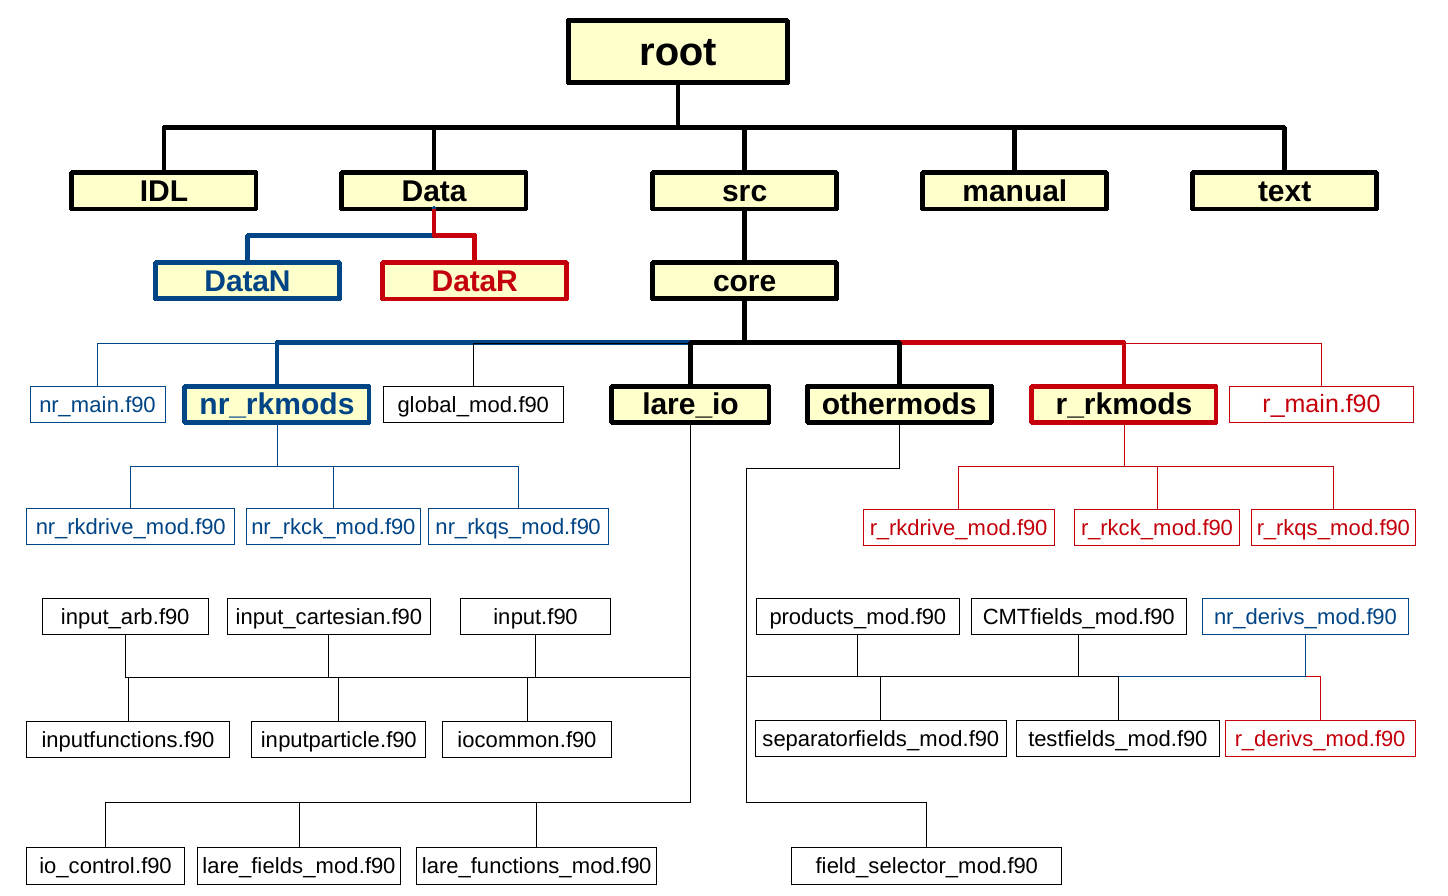
\includegraphics[width=0.85\textwidth]{rnrcode_layoutv2.png}
 \caption{code layout; filled rectangles represent folders, blue items are components of the non-relativistic code, while red items are components of the relativistic code; black represents general (global) files/folders used by both codes.} 
 \label{fig:codelayout}
\end{figure*}
\noindent In its present state, the code can easily be switched between separator, CMT, test or LareXd model fields using the \texttt{FMOD} variable in \texttt{global\_mod.f90}. Switching between models requires the code to be remade. Compilation and Makefile contents are discussed in more detail in Sec.~\ref{sec:Makefile}.

\section{Control deck: newinput.dat}\label{sec:controldeck}
Many of the input parameters for the code are specified in a control deck, located at \texttt{newinput.dat}. The contents of this file are read as an array, for which character spacing is important; in its current format, one cannot place comments in the control deck. The simplest way to explain how to set up a problem using this file is to go through the control deck line-by-line. A line from the code will be seen in \texttt{courier} font. \hspace{2mm}\\ 

\noindent The file begins with the line\\
\noindent\texttt{\&inputdata}\\
which begins the array of input data.\hspace{2mm}\\
\noindent\texttt{T1=105.}\\
\texttt{T2=200.}\\
The first variable to be specified is time, which runs from \texttt{T1} to \texttt{T2} and is in seconds (provided $\tscl$ is also defined in seconds). To avoid complications for the CMT model, the initial time \texttt{T1} is usually set to a value greater than $100\rm{s}$. For the separator reconnection field setup, we retain this view (for simplicity) and subtract \texttt{T1} from every time in the problem. For the current values of \texttt{T1} and \texttt{T2}, the code would run from $0\rm{s}$ and last approximately $95\rm{s}$ (\texttt{T2}$-$\texttt{T1}).\\
\noindent\texttt{H1=0.00001}\\	
\texttt{EPS=1.0E-15}\\
Of the next two values, \texttt{H1} represents the initial step-size for use with the RK algorithm, while \texttt{EPS} is a tolerance for the RK solvers. Increasing either value will increase the speed at which the code yields a solution, but with a trade-off in accuracy.\\
\noindent\texttt{AlphaSteps=2}\\
\texttt{AlphaMin=45.0}\\
\texttt{AlphaMax=45.0}\\
We now begin specifying particle parameters. The first is $\alpha$, the initial pitch angle distribution for our set of particles. \texttt{Alphasteps} specifies the (integer) number of times the range of $\alpha$ is divided, between an upper and lower bound (\texttt{Alphamin} and \texttt{Alphamax}, both in degrees). For unspecified reasons, setting \texttt{Alphasteps}$=2$ yields only one value of $\alpha$ for all the particles in the experiment. Increasing \texttt{Alphasteps} above two will cause the range to divide, between the upper and lower bounds (effectively, there are \texttt{Alphasteps}$-1$ particles in $\alpha$ space). 
\noindent$\alpha$ represents how the initial energy is divided between perpendicular and parallel components; $\alpha\sim0^{o}$ will cause all the energy to go to velocity along the magnetic field lines, while $\alpha\sim90^{o}$ will cause all the energy to go into perpendicular motion. In addition, $\alpha\sim180^{o}$ will also cause entirely parallel motion, but in the opposite direction to the direction of the magnetic field.\\
\noindent\texttt{R1(1)=-0.25E2}\\
\texttt{R2(1)=0.25E2}\\
\texttt{RSTEPS(1)=16}\\
We then create three 3-element arrays, containing the start, end and number of positions in $x,y,z$ space. The first three lines above are to specify where the grid of $x$ starts, ends, and how many positions in between these two values. The range \texttt{R2(1)}$-$\texttt{R1(1)} is divided by \texttt{RSTEPS(1)} divisions. Thus if \texttt{RSTEPS(1)}$=1$, then every particle in the experiment will begin at the same position in $x$. If \texttt{RSTEPS(1)}$=2$, then the two possible values of $x$ are \texttt{R1(1)} and \texttt{R2(1)}, respectively. In the above example, 16 positions from $-25\rm{m}\leq x\leq25\rm{m}$ are chosen (provided the lengthscale, $\lscl$, is also specified in metres). \texttt{R1} and \texttt{R2} are real values, while \texttt{RSTEPS} {\bf{must}} be an integer.\\
\noindent\texttt{R1(2)=-0.25E2}\\
\texttt{R2(2)=0.25E2}\\
\texttt{RSTEPS(2)=16}\\
Similarly the initial $y$ positions have been chosen, for \texttt{RSTEPS(2)} particles from minimum \texttt{R1(2)} to maximum \texttt{R2(2)}.\\
\noindent\texttt{R1(3)=-2.0E7}\\
\texttt{R2(3)=0.0E7}\\
\texttt{RSTEPS(3)=5}\\
Finally, the initial $z$ positions are chosen, distributed from \texttt{R1(3)} to \texttt{R2(3)}, \texttt{RSTEPS(3)} times.\\
\noindent\texttt{EkinLow=2e2}\\
\texttt{EkinHigh=2e2}\\
\texttt{EkinSteps=1/}\\
The final parameter to be chosen is the initial kinetic energy. Once again, it is possible to set this to a single value (as shown above) or for a range of initial kinetic energies. Unless otherwise specified, the values of \texttt{EkinLow} and \texttt{EkinHigh} are in units of $\rm{eV}$.\\


\noindent The \texttt{newinput.dat} control deck only controls the initial particle parameters. These values must be compatible with the other constants chosen in \texttt{global\_mod.f90}; the code will terminate if (for example) the initial particle positions are beyond the boundary specified by $x_{\rm end},y_{\rm end},z_{\rm end}$.
It is worth noting that altering values held in \texttt{newinput.dat} does {\bf{NOT}} require a code recompilation before re-running the code. However, if you intend to reduce the number of particles for the next simulation, remember that you may be left with additional output datafiles from previous runs, which might cause problems when you come to analyse your (now unexpectedly large) dataset.

\section{Makefile}\label{sec:Makefile}
The code is written using Fortran 90, and should work on all compilers which support this standard. However, the LareXd interface routines are written in MPI; LareXd datafiles are structured using blocks, not records. Therefore, for simplicity, the code is compiled against MPI compilers, such as mpif90.\\
%The current setup uses gfortran, but has also been compiled using ifort recently. The code is serial, hence MPI is not currently required to compile and run the code. 
To compile the code, simply type\\
\texttt{make}\\
which will compile both the non-relativistic and relativistic codes (using the default supplied compiler flags), and generate two binaries called\\
\texttt{bin/nrtest}\\
and\\
\texttt{bin/rtest}\\
The non-relativistic code can then be run on a workstation by typing\\
\texttt{./bin/nrtest}\\
at the command line, while\\
\texttt{./bin/rtest}\\
will run the relativistic code. It is possible to compile and run one version of the code without the other. By typing\\
\texttt{make ./bin/nrtest}\\
the Makefile will only compile the non-relativistic code. Similarly\\
\texttt{make ./bin/rtest}\\
yields only the binary containing the relativistic code.\\
The default data directory specified in the Makefile is \texttt{/Data}, with the non-relativistic data being output to \texttt{/Data/DataN} and relativistic data being output to \texttt{/Data/DataR}; if these settings are changed in the Makefile, be sure to update the output data character(s) in the \texttt{/src/core/global\_mod.f90} file before you try to run the code. By default, the binary files are automatically placed in the \texttt{./bin} subdirectory, while the compiler intermediate files go into the \texttt{obj} subdirectory.\\ 
\noindent To remove the compiled binaries, and the compiler intermediate files, type\\
\texttt{make clean}\\
\noindent To remove the intermediate files only, type\\
\texttt{make tidy}

\subsection{Makefile details}
The included Makefile is relatively complex and the main working parts should not be changed without a specific reason. However, it is possible for the user to customise various parts of the Makefile for several different reasons. The first customisable option is the compiler flags:
\begin{verbatim}
# Set the compiler flags 
#FFLAGS = -C -g -traceback -check all -warn all # mpif90 error flags
FFLAGS = -O3 
\end{verbatim}
The \texttt{FFLAGS} environment variable is used to control the general command line parameters passed to the MPIFortran compiler. 

\begin{itemize}
 \item\texttt{-O3} is a portable general purpose flag for turning on most optimisations on most machines.
 \item\texttt{-C} tests for attempts to write outside the bounds of an array and will print the location of the error and the name of the array which causes the problem (again good for debugging, but turns off {\bf{ALL}} compiler optimisation).
 \item\texttt{-g} places symbolic debugging information in the executable. This is sometimes useful, but often just annoying.
 \item\texttt{-traceback} enables a stack trace if the program crashes.
 \item\texttt{-check all} performs all runtime checks (includes bounds checking) can be useful when debugging but can slow down compilation and runtime, which can be annoying when you are sure the code works satisfactorily.
 \item\texttt{-warn all} tells gfortran to generate warnings about all common sources of bugs. Also falls into useful but annoying category.
\end{itemize}
\noindent The current settings reflect a successfully working code that requires no error checking. Switching between the two values of \texttt{FFLAGS} seen above may be useful when setting up a new problem, but can severely limit code performance if the debugging options are left on.

\begin{verbatim}
# Set some of the build parameters
TARGETN = nrtest
TARGETR = rtest
\end{verbatim}
\texttt{TARGETN} and \texttt{TARGETR} control the name of the output binary files in the \texttt{bin} subdirectory. Normally, there is no need to change this.\\
\begin{verbatim}
DATDIR = Data
\end{verbatim}
One may also change the output directory (for example, re-running the same experiment using a different field configuration); this is altered using the \verb|DATDIR| variable (but making sure that the 

\section{Output}\label{sec:output}
We will now discuss the output from the code, and how one extracts scientific information from it.
\subsection{IDL}
The IDL routines used for loading/visualising data are all held within the IDL directory. The most useful one (upon which everything else is build) is \texttt{getdata.pro}, which takes a given particle in the grid, and loads the data from a specific particle into a given data structure. The remaining procedures in \texttt{IDL/} are used to set up various aspects of 3D visualisation, and are included as a cheeky bonus!

\subsubsection{Starting IDL}
In order to load in the IDL routines, the IDL script \texttt{Start.pro} needs to be run. This can be run from the command line on starting IDL:
\begin{verbatim}
$ idl Start.pro
\end{verbatim}

\subsubsection{\texttt{getndata} and \texttt{getrdata}}
These functions load the data for a given particle number, for both relativistic and non-relativistic schemes. We will focus only on the non-relativistic code here; the syntax and usage for the relativistic version is identical. The syntax is:
\begin{verbatim}
IDL>  ds = getndata(a[,/flag1,...,/empty,wkdir=directory])
\end{verbatim}
After running this \texttt{ds} will contain the snapshot data structure for the (non-relativistic) code. Here, \texttt{a} is the number associated with the datafile you wish to load. Keeping in mind that there is no zeroth particle, providing a particle number \texttt{a} will initially only provide the position and time information from the \texttt{RV``a''.dat} file. If you wish to load additional quantities into the data structure \texttt{ds}, you must specify additional flags to the \texttt{getdata} call. To load all the variables, you can use the \texttt{/all} switch, i.e.
\begin{verbatim}
IDL>  ds = getndata(1,/all)
\end{verbatim}
will load all the variables associated with the first particle in the array of parameter space defined in \texttt{newinput.dat}.
The \texttt{wkdir=} option allows data to be loaded from a directory other than \texttt{/Data}, i.e. in the first example \texttt{directory} should be replaced with a string containing the name of the directory.
Some further examples:
\begin{verbatim}
IDL>  ds = getndata(10)
\end{verbatim}
This will only load the position and time variables for the 10th particle in the default data directory \texttt{Data}.
\begin{verbatim}
IDL>  ds = getndata(7,/fields,wkdir="OtherDir")
\end{verbatim}
In addition to $x,y,z,t$, this will also load $B_x, B_y, B_z$ and $E_x, E_y, E_z$ from particle 7 in the data directory \texttt{OtherDir} into the structure.
The various optional flags (and their related quantities) are defined in Table~\ref{tab:datastructure}.

\subsection{IDL Structure Tips}\label{subsec:IDLtips}
This section gives a brief overview of how to use IDL structures. The easiest way of doing this is with an example, to create the data structure:
\begin{verbatim}
IDL>  ds = getndata(1, /all)
\end{verbatim}
To view the elements contained in a structure the \texttt{help} command can be used with the \texttt{/struct} flag:
\begin{verbatim}
IDL> help, ds, /str
** Structure <11d16b68>, 16 tags, length=52000, data length=52000, refs=1:
   NAME            STRING    '../Data/RV00000001.dat'
   T               DOUBLE    Array[342]
   X               DOUBLE    Array[342]
   Y               DOUBLE    Array[342]
   Z               DOUBLE    Array[342]
   VPAR            DOUBLE    Array[342]
   MUBSQUARED      DOUBLE    Array[342]
   RDOTPERP        DOUBLE    Array[342]
   B               DOUBLE    Array[3, 342]
   E               DOUBLE    Array[3, 342]
   E2              DOUBLE    Array[342]
   E3              DOUBLE    Array[342]
   EK              DOUBLE    Array[342]
   GYROF           DOUBLE    Array[342]
   GYROP           DOUBLE    Array[342]
   GYROR           DOUBLE    Array[342]
\end{verbatim}
Ignore the first line. The rest of the lines are the elements, the variable type and (if the variable is an array) the array dimensions or the data value. 
To access the elements use \texttt{datastructure.element}, for example to print the filename:
\begin{verbatim}
IDL> print, ds.name
../Data/DataN/RV00000001.dat
\end{verbatim}

\subsection{Variable tables}
The code will, by default, only output certain variables for a single particle over the course of the simulation. It is also possible to use the \texttt{/all} switch to output all the variables into the required structure. A catalog of all the system variables (including the switches required to output them via \texttt{getdata}) can be found in Table~\ref{tab:datastructure}.

\begin{table}[ht]
\begin{flushleft}
\begin{tabular}{|c|p{0.7\columnwidth}|}
\multicolumn{2}{l}{{\bf Default variables:}}\\
\multicolumn{2}{l}{{\em These are all included in a standard \texttt{getdata} call.}}\\
\hline
name& String containing the filename of the file the data was loaded from.\\
t& Array containing the time of each output dump.\\
x& Array containing the $x$ coordinate of the particle at each output dump.\\
y& Array containing the $y$ coordinate of the particle at each output dump.\\
z& Array containing the $z$ coordinate of the particle at each output dump.\\
\hline
\end{tabular}
\vspace{0.5cm}\\
\begin{tabular}{|c|p{0.6\columnwidth}|l|}
\multicolumn{3}{l}{{\bf Simulation variables:}}\\
\multicolumn{3}{l}{{\em Additional variables are included using \texttt{/all} or individual switches.}}\\
\hline
Name&Description&Switch.\\
\hline
B&Three components of the magnetic field $(B_x,B_y,B_z)$.& \texttt{/fields}.\\
E&Three components of the electric field $(E_x,E_y,E_z)$.& \texttt{/fields}.\\
vpar&Array containing the parallel component of velocity, $v_\parallel$.& \texttt{/vpar}.\\
epar&Array containing the parallel Electric field, $\Epar$.& \texttt{/epar}.\\
muB&Array containing $\mu B=1/2m\vperp^2$. &\texttt{/muB}.\\
rdotperp& Perpendicular displacement velocity, $|\dot{\bf{R}}_\perp|$. & \texttt{/rdotperp}.\\
gyrof& The gyrofrequency, $\Omega$ as a function of time. & \texttt{/gyro}.\\
gyrop& The gyroperiod, $1/\Omega$, as a function of time. & \texttt{/gyro}.\\
gyror& The gyroradius, $r_g$, as a function of time. & \texttt{/gyro}.\\
ue& Three components of ${\bf{E}}\times{\bf{B}}$ drift velocity. & \texttt{/drift}.\\
e2& Energy associated with the magnetic moment, $\mu|{\bf{B}}|$. & \texttt{/ke}.\\
e3& Energy of the ${{E}}\times{{B}}$ drift velocity. & \texttt{/ke}.\\
ek& The total kinetic energy of the particle ($e2+e3+1/2m\vpar^2$). & \texttt{/ke}.\\
\hline
\end{tabular}
\begin{tabular}{|c|p{0.6\columnwidth}|l|}
%\multicolumn{3}{l}{{\bf Additional Relativistic Simulation variables:}}\\
\multicolumn{3}{l}{{\em only active using \texttt{getrdata.pro}}}\\
\hline
Name&Description&Switch.\\
\hline
gamma&Lorentz factor $\gamma$.& \texttt{/rel}.\\
upar&Parallel component of relativistic velocity $\upar(=\gamma\vpar)$& \texttt{/rel}.\\
ek& The total kinetic energy of the particle $\gamma m_0c^2$. & \texttt{/ke}.\\
\hline
\end{tabular}
\end{flushleft}
\caption{List of all the elements of the data structure and a brief description.}
\label{tab:datastructure}
\end{table} 

\subsection{3D data visualisation with IDL}
In addition to some custom routines to read in the data from the output files, we have also included routines to allow the user to visualise magnetic fields, particle paths and quantities in 3D space. The \texttt{Start.pro} file will load in several different subroutines to assist with this process. This is very much still work-in-progress; we will outline some basic features of some routines. It is likely we will also include several example programs with these routines, in order to show how one might use them to study specific quantities or problems. The objective of this section is to show what is possible, {\bf{not}} to document {\bf{every}} routine in the \texttt{IDL} directory, so be warned!

\subsubsection{Basic plot tools}
Before we describe more complex programs, we will first briefly outline some basic 3D plotting tools. Many of our codes make use of the intrinsic IDL routine \texttt{xplot3d}. This creates an interactive 3D graphics object. For example, having read in a series of particle positions using \texttt{getndata} or \texttt{getrdata}, we may plot the trajectory of the particle using 
\begin{verbatim}
IDL> xplot3d, ds.x, ds.y, ds.z
\end{verbatim}
which yields a 3D interactive particle path as shown in Fig.~\ref{fig:simples}.
 \begin{figure}[t]
   \centering
   \resizebox{0.4\textwidth}{!}{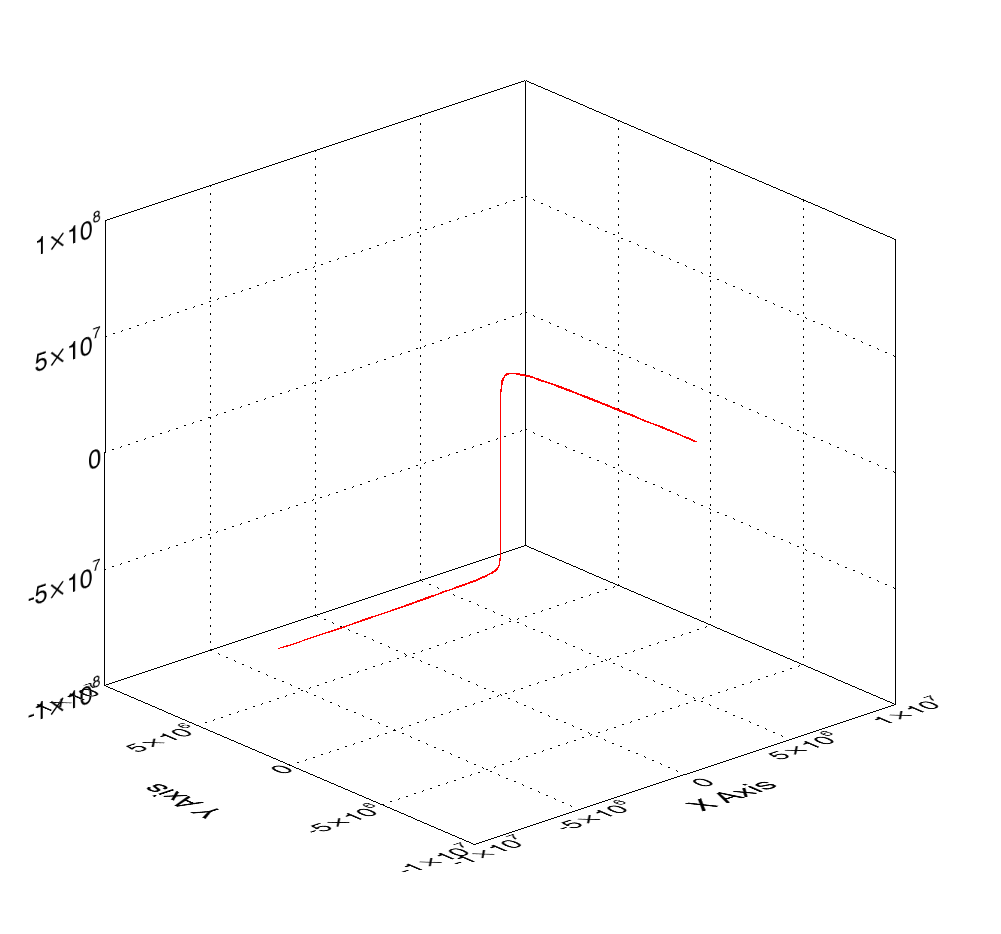
\includegraphics{manual1.png}} 
   \resizebox{0.27\textwidth}{!}{
\includegraphics{manual2.png}}
   \resizebox{0.27\textwidth}{!}{
\includegraphics{manual3.png}} 
   \caption{Example of basic plot tools used in more complicated routines; a single particle path as shown in \texttt{xplot3d}, together with two 3D graphics objects we will use in our routines; orbs and vectors.} 
   \label{fig:simples}
 \end{figure}
\texttt{xplot3d} can also overlay certain 3D symbols at certain positions. In order to display scalar quantities or specific positions, we will use IDL to create orbs, in the following manner
\begin{verbatim}
IDL> orb = OBJ_NEW('orb', COLOR=[255, 0 ,0])
IDL> osym = OBJ_NEW('IDLgrSymbol', oOrb)
\end{verbatim}
This stores a red orb as a 3D symbol, ready to be overlaid into \texttt{xplot3d} (shown in the central panel of Fig.~\ref{fig:simples}). Using a custom routine, one can also generate arrow symbols, in order to specify vector quantities at a given position. This is done using the \texttt{mk\_vector} routine, and is used as follows
\begin{verbatim}
IDL> oModel=obj_new('IDLgrModel')
IDL> oModel->add,mk_vector([1,1,1],color=[0,0,255])
IDL> asym = OBJ_NEW('IDLgrSymbol', oModel)
\end{verbatim}
which generates a blue arrow, extending one unit in $x$, $y$, and $z$ (see right panel of Fig.~\ref{fig:simples}). Placing either symbol at a specific position requires the use of the  \texttt{symbol} keyword in \texttt{xplot3d}. If we wanted to overlay each symbol at a certain position on the previous diagram, for example, we might use 
\begin{verbatim}
IDL> xplot3d, [x1,x1], [y1,y1],[z1,z1], SYMBOL=osym, /OVERPLOT
IDL> xplot3d, [x2,x2], [y2,y2],[z2,z2], SYMBOL=asym, /OVERPLOT
\end{verbatim}
where $(x1,y1,z1)$ and $(x2,y2,z2)$ are the positions of the centre of the orb and the base of the arrow. Many of the codes which follow build on these simple initial principles. [NB. one should ensure the symbols are rescaled to match the plot range specified in \texttt{xplot3d}].

\subsubsection{\texttt{ODEINT}}
It is often useful to display the magnetic field in the simulation at a given time. We already know the equations which describe the field (Eqs.~\ref{subeq:B0}-\ref{subeq:B}); like good mathematicians, we can easily solve for the fieldlines in 3d space by solving the coupled set of ODEs:
\[
 \frac{ds}{B}= \frac{dx}{B_x}= \frac{dy}{B_y}= \frac{dz}{B_z}, \qquad B=|{\bf{B}}|=\sqrt{B_x^2+B_y^2+B_z^2}.
\]
The \texttt{ODEINT.pro} program solves this coupled set of ODEs for an initial position in $x,y,z$ space using another RK algorithm (with the field specified in the \texttt{derivs} subroutine). \texttt{ODEINT} outputs a set of positions in $x,y,z$ which traces out the location of a single field line (a line of constant magnetic flux).

\subsubsection{\texttt{FLINE}}
To show the global structure of the magnetic field, we can make repeated use of \texttt{ODEINT} for a grid of initial positions, in a program called \texttt{FLINE.pro}. This essentially creates a grid of initial positions, and repeatedly calls \texttt{ODEINT} for each specified position. \texttt{FLINE} also makes use of the \texttt{mk\_vector} subroutine (to draw arrows in the direction of the magnetic field) and IDL orbs (to indicate the locations of the magnetic null points). 
All the options (the initial starting positions for the \texttt{ODEINT} routine, symbols and colours, 3D plotting area etc) are all specified within the routine itself. To run, simply type
\begin{verbatim}
IDL> FLINE
\end{verbatim}
which should yield a 3D interactive object like those seen in Fig.~\ref{fig:myfield}. It is worth noting that the examples shown in this image are for the initial (potential) field only ($t=0$). The \texttt{FLINE} program is also capable of plotting the magnetic field lines at {\bf{any}} time ($0\leq t\leq \tau$).
   \begin{figure*}[t]
    \centering
    \subfloat[\texttt{FLINE} example 1.]{\label{subfig:field1}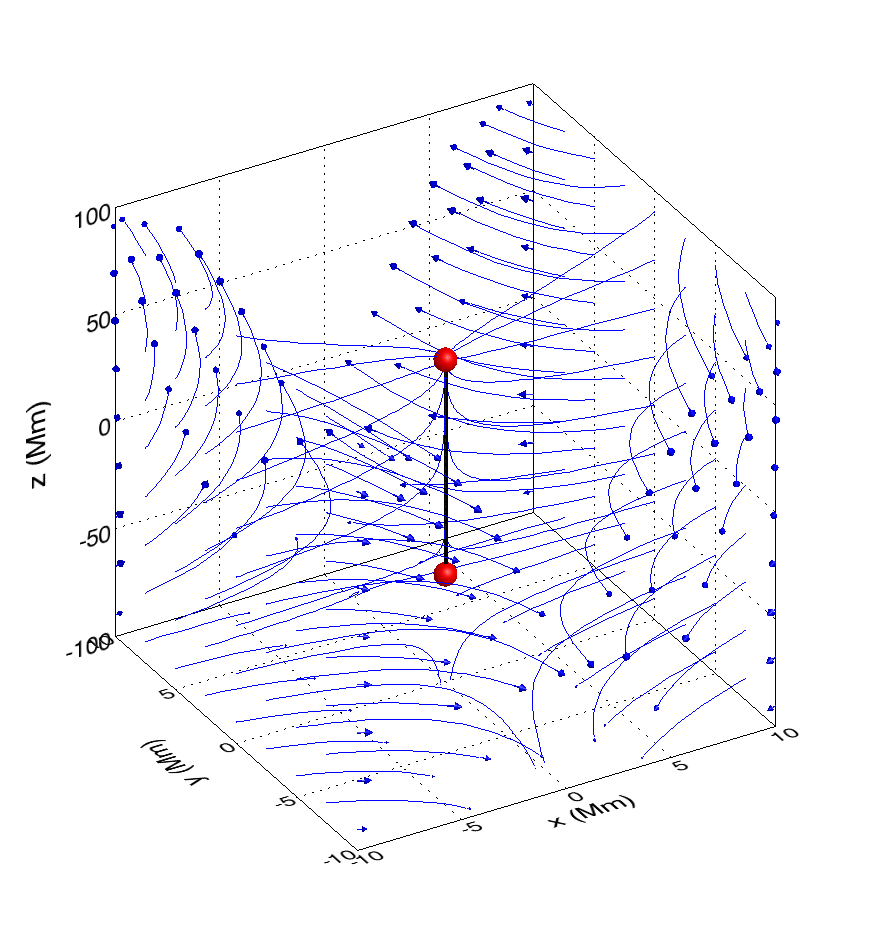
\includegraphics[width=0.45\textwidth]{iniB_plusnullsep.png}}
    \subfloat[\texttt{FLINE} example 2.]{\label{subfig:field2}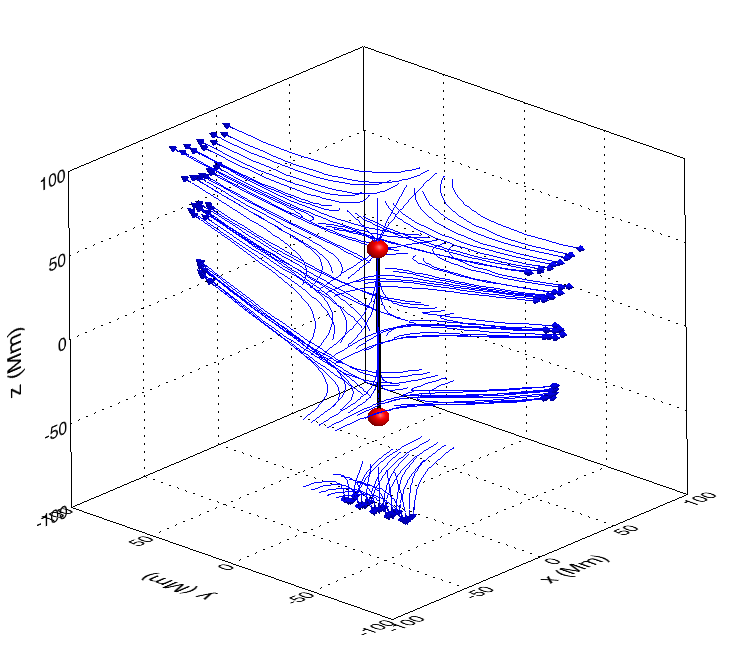
\includegraphics[width=0.53\textwidth]{iniB_plusnullseplarge.png}}
    \caption{Illustration of selected field lines given by Eq.~\ref{subeq:B0}, comparing local magnetic field and orientation (blue) relative to the location of the two nulls (red) connected by a separator (black), over two different ranges in $x,y$, using \texttt{FLINE}.} 
    \label{fig:myfield}
   \end{figure*}

\subsubsection{\texttt{particletrack} and \texttt{iniorb}}
To streamline the process of reading in data from individual particles and displaying this information on screen, we have created a routine called \texttt{particletrack}. This routine automatically reads in and displays/overlays the particle position as a function of time, together with optional extras (initial and final particle positions, locations of bounce points, colour of field line depends on some quantity, lengthscales of global plot, etc) using a single command.
For example, to draw the trajectory of the 55th particle in the simulation, one need only type 
\begin{verbatim}
IDL> particletrack, 55, xyzt
\end{verbatim}
where a 1024 element particle path is output to a variable called \texttt{xyzt} automatically. One can then build up several of these paths in the same window, using the \texttt{op} switch. For example
\begin{verbatim}
IDL> particletrack, 65, xyzt, /op
\end{verbatim}
would overplot the 65th particle path on to the already created window. 
\begin{verbatim}
IDL> particletrack, 75, xyzt, /op, /bsymb, /symb, lcol=[153,0,153]
\end{verbatim}
would overlay the 75th particle track (in purple), a blue orb at locations where the parallel velocity of the particle ($\vpar$) changes sign, a green orb at the initial location of the particle, and a red orb at the position of the particle when the simulation ends. 

We have also created a similar routine to just display the initial positions of every particle, using orbs, called \texttt{iniorb}. It is called using exactly the same syntax as \texttt{particletrack}.

By repeatedly looping calls to the \texttt{particletrack} and \texttt{iniorb} routines, one can build up a picture of global trends in particle behaviour. This is demonstrated in Fig.~\ref{fig:ptexample}, where \texttt{particletrack} is used to display the paths and \texttt{iniorb} the initial positions of 1280 particles, in order to identify trends in the data.
\begin{figure}[th]
 \centering
 \subfloat[particle tracks]{\label{subfig:egtrack}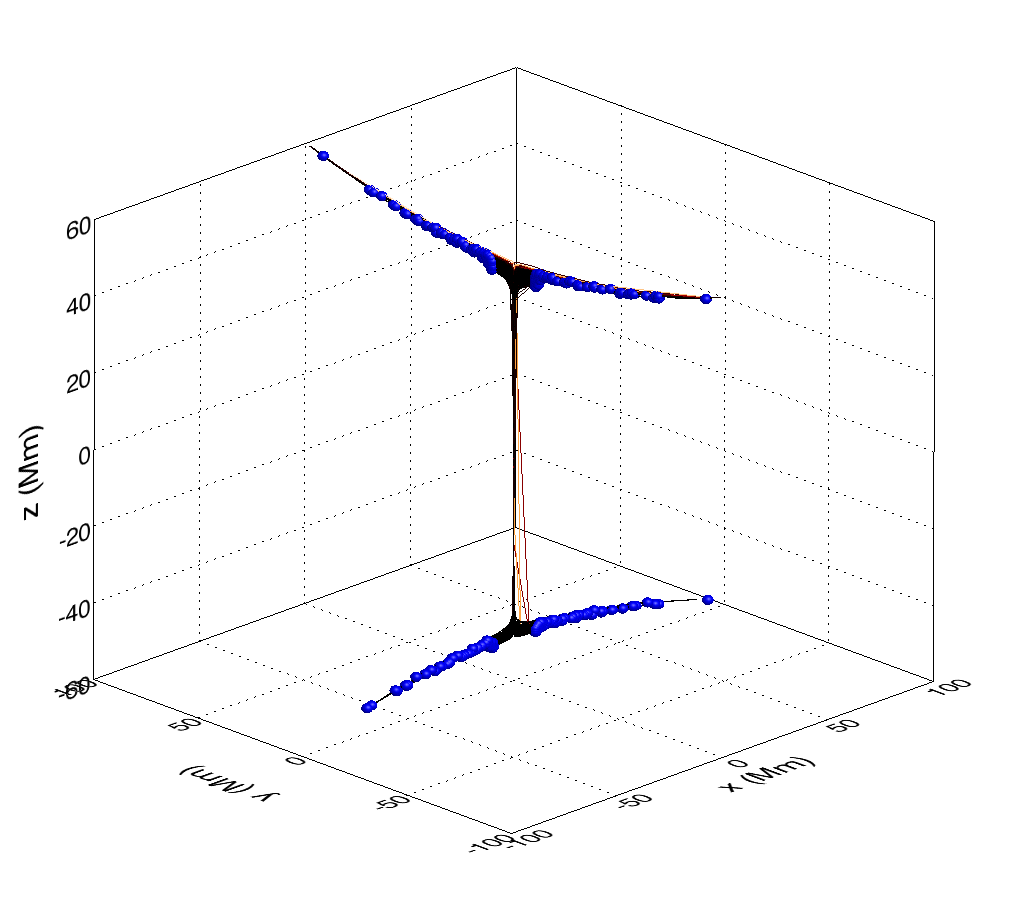
\includegraphics[width=0.42\textwidth]{final_particletracks.png}} 
 \subfloat[initial positions]{\label{subfig:egpos}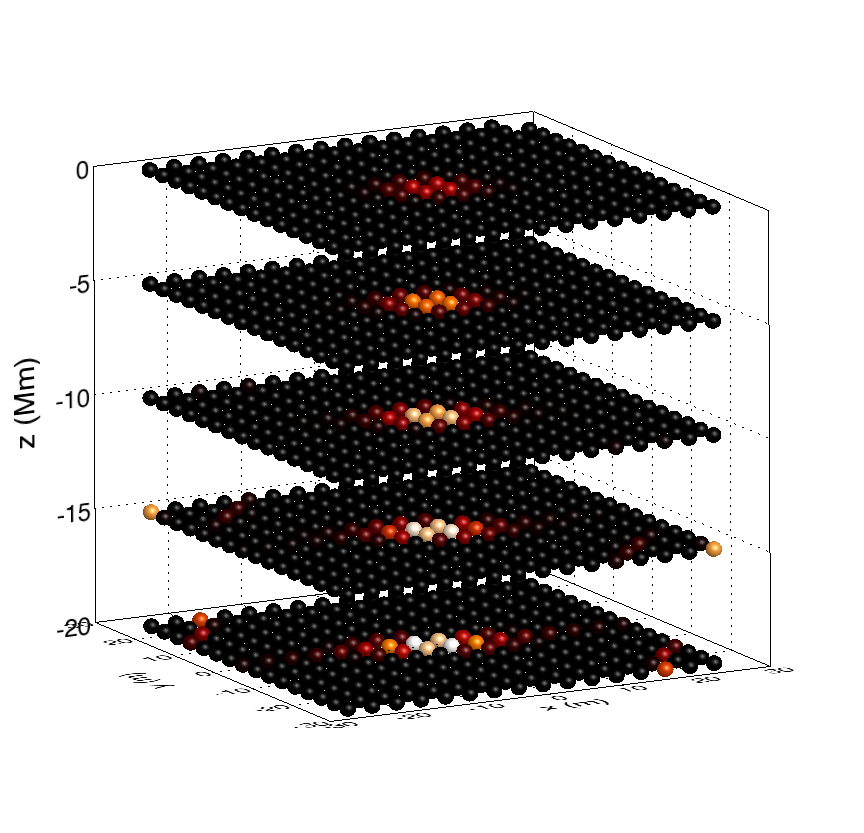
\includegraphics[width=0.39\textwidth]{final_particlepositions.png}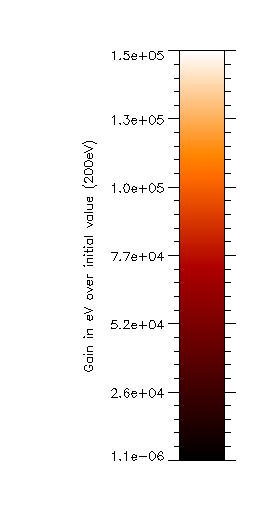
\includegraphics[width=.18\textwidth]{final_colourscale.png}} 
 \caption{Global behaviour example; \protect\subref{subfig:egtrack} shows particle trajectories (and mirror points), while \protect\subref{subfig:egpos} shows initial positions, all coloured to identify differences in particle behaviour. This example highlights the peak energy gained by individual particles during the simulation (see colour bar for specific values).}
 \label{fig:ptexample}
\end{figure}


\section{Common Questions}

\subsection*{How can I create a second copy of my executed code, without also copying the datafiles?}
I've found that entering the following on the command line can help with this:\\
\texttt{find . -depth ! -name ``RV*.dat'' | cpio -pdmv ../newfolder}\\
The command finds all files within a given directory (and subdirectories), and copies them to a new folder whilst omitting those whose name matches \texttt{RV*.dat} from the copy. Isn't that nifty?

\subsection*{How do I delete old data that I no longer want?}
The Makefile option\\
\texttt{make clean}\\
will not remove any output data, but will simply reset/delete the executable files. However, typing\\
\texttt{make datatidy}\\
should remove the datafiles present in the \texttt{/Data} subdirectory without doing anything to the code. This is effectively equivalent to\\
\texttt{rm -rf Data/*}\\
but I tend to panic when the \texttt{-f} flag is active on the remove command, so be careful if you do this manually!

\subsection*{What are all the extra files in the folder \texttt{IDL/JTfiles}?}
This code is a work in progress. I am currently using this code as part of my postdoctoral research. Many of these codes have been written to solve/address specific issues, show specific quantities and how they change during the simulation. Many are simply wrappers for codes like \texttt{particletrack}, so that you can see how to repeatedly call those routines in a given setup. I have also toyed with adding various different 3D interactive symbols in one or two codes. How you use these additional codes is up to you, but I have included them as a reference for the time being to show what is possible.

\pagebreak
\newpage
 \bibliographystyle{plainnat.bst}
 \bibliography{manual} 
\end{document}


